\begin{frame}{Energy-based self-supervised representation learning}

  \begin{align*}
    similarity(x_{i}, x_{j}) > similarity(x_{i}, x_{k}) \Rightarrow energy(e_{i}, e_{j}) < energy(e_{i}, e_{k})
  \end{align*}

  \begin{figure}
    \includegraphics[width=0.4\textwidth]{energy_siamese}
  \end{figure}

  \note{
    \begin{itemize}
      \item For energy-based learning we often use what is called Siamese networks.
      \item Two (almost) identical networks, that share weights.
      \item We could summarize the methods in this chapter also as Siamese Representation Learning.
      \item If the inputs to the two networks are compatible in some way, the energy should be low, otherwise high.
      \item Similarity does not mean similar appearance in pixel space.
    \end{itemize}
  }

\end{frame}


\begin{frame}{Contrastive Learning}

  \begin{figure}
    \includegraphics[width=0.9\textwidth]{pirl}
  \end{figure}

  \note{
    \begin{itemize}
      \item Image from Self-Supervised Learning of Pretext-Invariant Representations, Misra \& Maaten, CVPR 2020
    \end{itemize}
  }

\end{frame}


\begin{frame}{Contrastive Learning}

  \begin{figure}
    \includegraphics[width=0.9\textwidth]{pirl_layers}
  \end{figure}

  \note{
    \begin{itemize}
      \item Image from Self-Supervised Learning of Pretext-Invariant Representations, Misra \& Maaten, CVPR 2020
    \end{itemize}
  }

\end{frame}


\begin{frame}{Contrastive Learning}

  \begin{figure}
    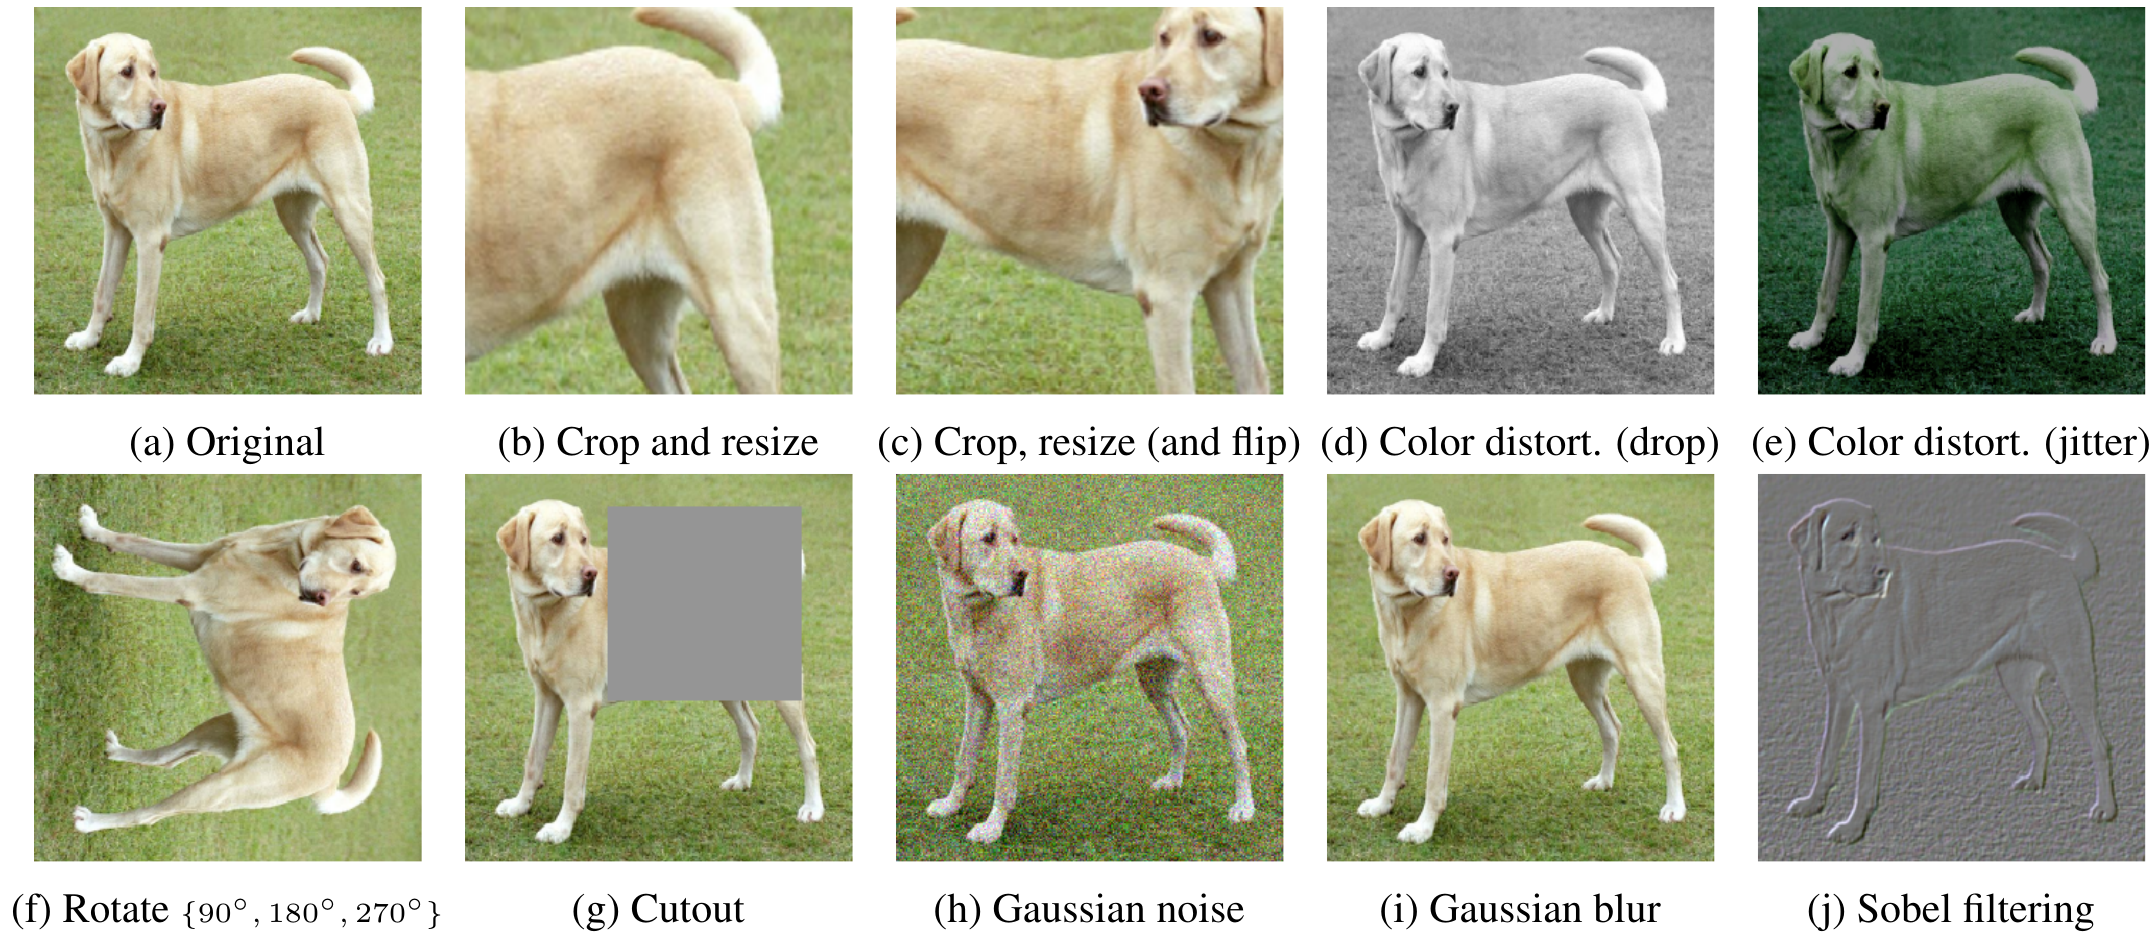
\includegraphics[width=0.9\textwidth]{simclr_distortions}
  \end{figure}

  \note{
    \begin{itemize}
      \item Image from A Simple Framework for Contrastive Learning of Visual Representation, Chen et al., ICML 2020
    \end{itemize}
  }

\end{frame}


\begin{frame}{Contrastive Learning}

  Good negative samples are very important
  \begin{itemize}
    \item Have huge batch sizes
    \item Use memory banks (momentum of activations)
    \item Momentum on the weights of the siamese twin
  \end{itemize}


  \note{
    \begin{itemize}
      \item Huge batch sizes are easy to implement but have heavy compute demands  \\
            A Simple Framework for Contrastive Learning of Visual Representations, Chen et al., ICML 2020
      \item Compute efficient but memory bank needs a lot of RAM \\
            Unsupervised Feature Learning via Non-Parametric Instance-level Discrimination, Wu et al., CVPR 2018
      \item Saves memory but needs extra forward pass \\
            Momentum Contrast for Unsupervised Visual Representation Learning, He et al., CVPR 2020
    \end{itemize}
  }

\end{frame}


\begin{frame}{Non-Contrastive Learning}

  There are other ways to approach this (clustering, distillation)
  \begin{itemize}
    \item DeepCluster, Sela, SwAV
    \item BYOL, SimSiam
  \end{itemize}

  \note{
    \begin{itemize}
      \item We are gonna skip those for today. Unfortunately we can't talk about everything :(
      \item There is a very nice lecture by Ishan Misra though, if you want to learn more: \url{https://www.youtube.com/watch?v=8L10w1KoOU8}
    \end{itemize}
  }

\end{frame}


\begin{frame}{Redundancy Reduction Learning}

  \begin{align*}
    f_{i}(I) &= f_{i}(d(I))\\
    f_{i}(I) &\neq f_{j}(d(I))
  \end{align*}

  \note{
    \begin{itemize}
      \item This equations are a dramatically oversimplified sketch of the idea.
      \item While neurons should respond the same to an image and its distorted version, they should all respond differently.
      \item We don't have spare neurons, so we don't want redundancy in their activations.
      \item Possible principles underlying the transformation of sensory messages, Horace Barlow, 1961
    \end{itemize}
  }

\end{frame}


\begin{frame}{Barlow Twins}

  \begin{figure}
    \includegraphics[width=0.9\textwidth]{barlow_twins}
  \end{figure}

  \note{
    \begin{itemize}
      \item Our objective is to make the correlation matrix a diagonal matrix.
      \item To prevent constant but decorrelated output, $Z_{a}$ and $Z_{b}$ are standardized before the correlation matrix is computed.
      \item Image from Barlow Twins: Self-Supervised Learning via Redundancy Reduction, Zbontar et al., ICML 2021
    \end{itemize}
  }

\end{frame}


\begin{frame}{Barlow Twins}

  \begin{figure}
    \includegraphics[height=0.9\textheight]{barlow_twins_algo}
  \end{figure}

  \note{
    \begin{itemize}
      \item Image from Barlow Twins: Self-Supervised Learning via Redundancy Reduction, Zbontar et al., ICML 2021
    \end{itemize}
  }

\end{frame}



% \begin{frame}{SEER}

%   \note{
%     \begin{itemize}
%       \item
%     \end{itemize}
%   }

% \end{frame}
